\documentclass[11pt,compress,t,notes=noshow, xcolor=table]{beamer}
\usepackage[]{graphicx}\usepackage[]{color}
% maxwidth is the original width if it is less than linewidth
% otherwise use linewidth (to make sure the graphics do not exceed the margin)
\makeatletter
\def\maxwidth{ %
  \ifdim\Gin@nat@width>\linewidth
    \linewidth
  \else
    \Gin@nat@width
  \fi
}
\makeatother

\definecolor{fgcolor}{rgb}{0.345, 0.345, 0.345}
\newcommand{\hlnum}[1]{\textcolor[rgb]{0.686,0.059,0.569}{#1}}%
\newcommand{\hlstr}[1]{\textcolor[rgb]{0.192,0.494,0.8}{#1}}%
\newcommand{\hlcom}[1]{\textcolor[rgb]{0.678,0.584,0.686}{\textit{#1}}}%
\newcommand{\hlopt}[1]{\textcolor[rgb]{0,0,0}{#1}}%
\newcommand{\hlstd}[1]{\textcolor[rgb]{0.345,0.345,0.345}{#1}}%
\newcommand{\hlkwa}[1]{\textcolor[rgb]{0.161,0.373,0.58}{\textbf{#1}}}%
\newcommand{\hlkwb}[1]{\textcolor[rgb]{0.69,0.353,0.396}{#1}}%
\newcommand{\hlkwc}[1]{\textcolor[rgb]{0.333,0.667,0.333}{#1}}%
\newcommand{\hlkwd}[1]{\textcolor[rgb]{0.737,0.353,0.396}{\textbf{#1}}}%
\let\hlipl\hlkwb

\usepackage{framed}
\makeatletter
\newenvironment{kframe}{%
 \def\at@end@of@kframe{}%
 \ifinner\ifhmode%
  \def\at@end@of@kframe{\end{minipage}}%
  \begin{minipage}{\columnwidth}%
 \fi\fi%
 \def\FrameCommand##1{\hskip\@totalleftmargin \hskip-\fboxsep
 \colorbox{shadecolor}{##1}\hskip-\fboxsep
     % There is no \\@totalrightmargin, so:
     \hskip-\linewidth \hskip-\@totalleftmargin \hskip\columnwidth}%
 \MakeFramed {\advance\hsize-\width
   \@totalleftmargin\z@ \linewidth\hsize
   \@setminipage}}%
 {\par\unskip\endMakeFramed%
 \at@end@of@kframe}
\makeatother

\definecolor{shadecolor}{rgb}{.97, .97, .97}
\definecolor{messagecolor}{rgb}{0, 0, 0}
\definecolor{warningcolor}{rgb}{1, 0, 1}
\definecolor{errorcolor}{rgb}{1, 0, 0}
\newenvironment{knitrout}{}{} % an empty environment to be redefined in TeX

\usepackage{alltt}
\newcommand{\SweaveOpts}[1]{}  % do not interfere with LaTeX
\newcommand{\SweaveInput}[1]{} % because they are not real TeX commands
\newcommand{\Sexpr}[1]{}       % will only be parsed by R



\usepackage[english]{babel}
\usepackage[utf8]{inputenc}

\usepackage{dsfont}
\usepackage{verbatim}
\usepackage{amsmath}
\usepackage{amsfonts}
\usepackage{bm}
\usepackage{csquotes}
\usepackage{multirow}
\usepackage{longtable}
\usepackage{booktabs}
\usepackage{enumerate}
\usepackage[absolute,overlay]{textpos}
\usepackage{psfrag}
\usepackage{algorithm}
\usepackage{algpseudocode}
\usepackage{eqnarray}
\usepackage{arydshln}
\usepackage{tabularx}
\usepackage{placeins}
\usepackage{tikz}
\usepackage{setspace}
\usepackage{colortbl}
\usepackage{mathtools}
\usepackage{wrapfig}
\usepackage{bm}
\usetikzlibrary{shapes,arrows,automata,positioning,calc,chains,trees, shadows}
\tikzset{
  %Define standard arrow tip
  >=stealth',
  %Define style for boxes
  punkt/.style={
    rectangle,
    rounded corners,
    draw=black, very thick,
    text width=6.5em,
    minimum height=2em,
    text centered},
  % Define arrow style
  pil/.style={
    ->,
    thick,
    shorten <=2pt,
    shorten >=2pt,}
}
\usepackage{subfig}


% Defines macros and environments
\input{../../style/common.tex}

%\usetheme{lmu-lecture}
\newcommand{\titlefigure}{figure/eval_mclass_roc_sp_13}
\newcommand{\learninggoals}{
\item Understand why pAUC is a reasonable metric in some contexts
\item Know how pAUC is computed and normalized
\item Understand multi-class AUC}
\usepackage{../../style/lmu-lecture}

\let\code=\texttt
\let\proglang=\textsf

\setkeys{Gin}{width=0.9\textwidth}

\title{Introduction to Machine Learning}
% \author{Bernd Bischl, Christoph Molnar, Daniel Schalk, Fabian Scheipl}
\institute{\href{https://compstat-lmu.github.io/lecture_i2ml/}{compstat-lmu.github.io/lecture\_i2ml}}
\date{}

\setbeamertemplate{frametitle}{\expandafter\uppercase\expandafter\insertframetitle}


\begin{document}


% This file loads R packages, configures knitr options and sets preamble.Rnw as parent file
% IF YOU MODIFY THIS, PLZ ALSO MODIFY setup.Rmd ACCORDINGLY...


% Defines macros and environments
\input{../../latex-math/basic-math.tex}
\input{../../latex-math/basic-ml.tex}
\input{../../latex-math/ml-automl.tex}
%! includes: basics-learners 

\lecturechapter{Evaluation: AUC Extensions}
\lecture{Introduction to Machine Learning}

% ------------------------------------------------------------------------------

\begin{vbframe}{Partial AUC}

\begin{itemize}
  \item Sometimes it can be useful to look at a specific region under the ROC 
  curve $\Rightarrow$ partial AUC (pAUC).
  % \item This leads to partial AUC (pAUC), originally proposed by 
  % \href{http://journals.sagepub.com/doi/pdf/10.1177/0272989X8900900307}
  % {McClish (1989)}.
  \item For example, we might focus on a region with low FPR or a region with 
  high TPR:
\end{itemize}

\begin{knitrout}\scriptsize
\definecolor{shadecolor}{rgb}{0.969, 0.969, 0.969}\color{fgcolor}
{\centering \includegraphics[width=0.9\textwidth]{figure/eval_mclass_roc_sp_13}}
\end{knitrout}

\end{vbframe}

% ------------------------------------------------------------------------------

\begin{vbframe}{Partial AUC -- example}

\begin{itemize}
  \item Applications where sensitivity and specificity are treated asymetrically 
  often occur in biomedical contexts.
  \item For example, 
  \href{https://clincancerres.aacrjournals.org/content/16/24/6111}
  {Wild et al. (2010)} used pAUC in their study of biomarkers for the detection 
  of colorectal cancer.
  \item Sensitivity, i.e., being able to correctly detect present diseases, is 
  crucial in this setting.
  \item At the same time, high sensitivity is only useful if the classifier also 
  achieves high specificity. \\
  $\rightarrow$ Otherwise, healthy patients might receive costly and entirely 
  unnecessary treatment.
  \item It is therefore reasonable to demand a certain level of specificity and 
  evaluate/optimize learners on the resulting pAUC.
\end{itemize}

\end{vbframe}

% ------------------------------------------------------------------------------

\begin{vbframe}{Corrected Partial AUC}

\begin{itemize}
  \item The scale of the partial AUC depends on the FPR cut-off values used to 
  determine the region of interest $\Rightarrow \text{pAUC} \in [0, c_2 - c_1]$.
  \item For standard AUC, we have $c_1 = 0$ and $c_2 = 1$.
  \item We can scale pAUC to take on values in $[0, 1]$ again:
  $$\text{pAUC}_\text{corrected} = \cfrac{1}{2} \left( 1 + \cfrac{\text{pAUC} - 
  \text{AUC}_{\text{min}}}{\text{AUC}_{\text{max}} - \text{AUC}_{\text{min}}} 
  \right),$$
  where
  \begin{itemize}
    \item $\text{AUC}_{\text{min}}$ is the value of the non-discriminant AUC, 
    and
    \item $\text{AUC}_{\text{max}}$ is the maximum possible AUC in the region.
  \end{itemize}
  % \item As usual, $\text{pAUC} = 0.5$ corresponds to the non-discriminant and 
  % $\text{pAUC} = 1$ to the perfect classifier.
  \lz
  \item NB: using pAUC means casting aside parts of the information 
  deliberately.
\end{itemize}

\end{vbframe}

% ------------------------------------------------------------------------------

\begin{vbframe}{Multi-class AUC}

% \small

\begin{itemize}
  \small
  \item In its original form, AUC (as the other ROC metrics) is defined for the 
  binary-class case.
  \item We can extend AUC to \textbf{multi-class} classification, where 
  estimating the area under the ROC curve evolves into estimating the 
  hypervolume under the ROC surface.
  \item This can be achieved by considering a set of two-dimensional curves, 
  resulting from binry comparisons, and subsequent aggregation. \\
  $\rightarrow$ In principle, we have the choice between one-vs-one and 
  one-vs-rest comparisons.
\end{itemize}  

\vfill
 
\begin{minipage}[c]{0.75\textwidth}
  \centering
  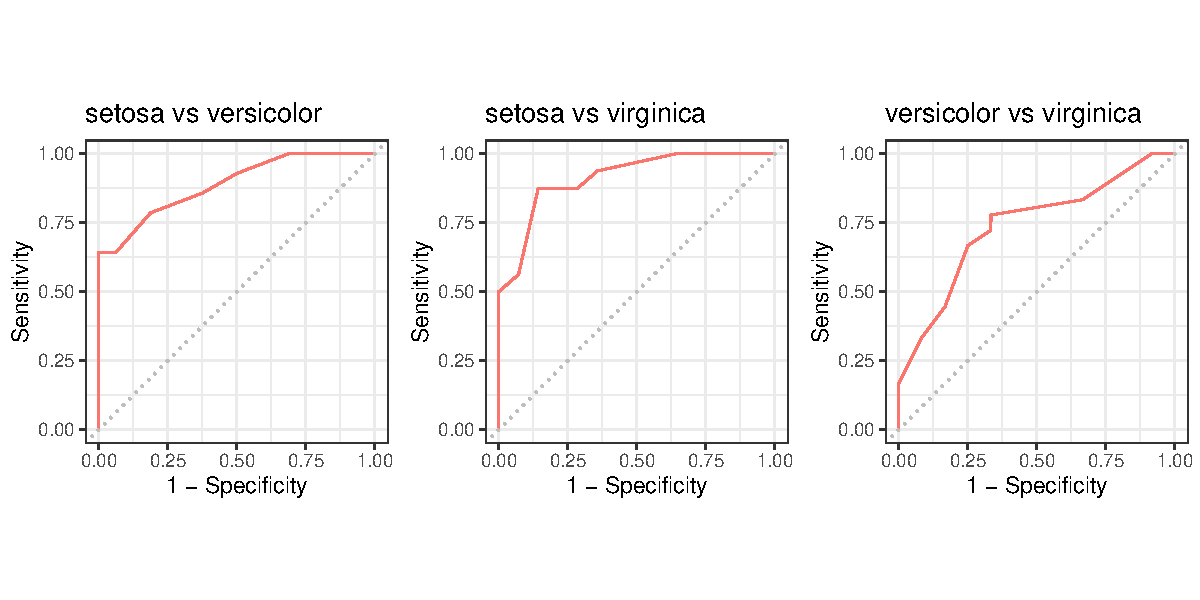
\includegraphics[trim = 0 40 -20 40, clip, width=\textwidth]
  {figure/eval_auc_extensions}
\end{minipage}%
\begin{minipage}[c]{0.25\textwidth}
  \scriptsize
  \raggedright
  One-vs-one comparisons between classes for classification of \texttt{iris} 
  species with LDA according to sepal width.
\end{minipage}
 
% \begin{center}
%   \includegraphics[trim = 0 40 0 40, clip, width=0.5\textwidth]
%   {figure/eval_auc_extensions}
% \end{center}
 
\framebreak
  
\begin{itemize}  
  \small
  \item For the first possibility, 
  \href{https://link.springer.com/article/10.1023/A:1010920819831}
  {Hand and Till (2001)} proposed to average the AUC of respective pairwise 
  comparisons between two classes.
  \begin{itemize}
    \small
    % \small
  % , where 
  % the classifier predicts the probability $\pik$ of belonging to class $k$ for 
  % each class $k \in \setg$.
  % \item \href{https://link.springer.com/article/10.1023/A:1010920819831}
  % {Hand and Till (2001)} proposed to average the AUC of pairwise comparisons 
  % (one-vs-one) of a multi-class classifier.
    \item First, compute for all pairs of classes $k, \ell \in \setg$ the 
    probability $\text{AUC}(k ~|~ \ell)$ of a randomly drawn member of class $k$ 
    having a lower probability of belonging to class $\ell$ than a randomly drawn 
    member of class $\ell$.
    \item For $g = 2$, we have $\text{AUC}(k ~|~ \ell) = 
    \text{AUC}(\ell ~|~ k)$, but not necessarily so for $g > 2$.
    \item However, since class identifiability is immune to any bijective 
    transformation of the labels, we cannot distinguish $\text{AUC}(k ~|~ \ell)$ 
    from $\text{AUC}(\ell ~|~ k)$, so we set 
    $\text{AUC}(k, \ell) = \frac{1}{2} \cdot [\text{AUC}(k ~|~ \ell) + 
    \text{AUC}(\ell ~|~ k)]$.
  
  % \begin{itemize}
  %   \item Compute $\text{AUC}(i,j)$ for each pair of classes $i, j \in \setg$.
  %   \item $\text{AUC}(i,j)$ is the probability that a randomly drawn member of 
  %   class $i$ has a lower probability of belonging to class $j$
  %   than a randomly drawn member of class $j$.
  %   \item For $g$ classes, we have ${{g}\choose{2}} = \tfrac{g (g-1)}{2}$ values 
  %   of $\text{AUC}(i,j)$, which are then averaged to compute the multi-class 
  %   AUC.
  % \end{itemize}
  
    \item Averaging over all pairs of classes yields the overall 
    $\text{AUC}_{MC}$ as a multi-class performance metric:
    $$\text{AUC}_{MC} = \frac{2}{g(g + 1)} \sum_{k < \ell} \text{AUC}(k, \ell) 
    \in [0, 1].$$
    \item This reduces to the standard AUC for the binary case.
    % \item Again, a non-discriminant classifier will have $\text{AUC}_{MC} = 0.5$
    % as all pairwise probability estimates equal 0.5.
  \end{itemize}
\end{itemize}
\end{vbframe}

% ------------------------------------------------------------------------------

\endlecture
\end{document}
